\documentclass{emulateapj}
%\documentclass[12pt,preprint]{aastex}

\usepackage{graphicx}
\usepackage{float}
\usepackage{amsmath}
\usepackage{epsfig,floatflt}
\usepackage{hyperref}
\usepackage[toc, page]{appendix}
\usepackage{verbatim, amsmath, amsfonts, amssymb, amsthm}
\usepackage[utf8]{inputenc}
\usepackage{textcomp}
\usepackage{float}
\usepackage{xcolor}
\usepackage{color}
\usepackage{listings}
\usepackage{fancyhdr}
\usepackage[T1]{fontenc}
\usepackage{url}
\usepackage[export]{adjustbox}
\usepackage{calc}

\usepackage{accents}
\newcommand{\dbtilde}[1]{\accentset{\approx}{#1}}
\newcommand{\vardbtilde}[1]{\tilde{\raisebox{0pt}[0.85\height]{$\tilde{#1}$}}}
\usepackage{lipsum, babel}
\usepackage{lipsum}
\usepackage[para]{footmisc}


\definecolor{mygreen}{rgb}{0,0.6,0}
\definecolor{mygray}{rgb}{0.5,0.5,0.5}
\definecolor{mymauve}{rgb}{0.58,0,0.82}

\lstset{ %
	backgroundcolor=\color{white}\ttfamily\tiny,   % choose the background color; you must add \usepackage{color} or \usepackage{xcolor}; should come as last argument
	basicstyle=\tiny,        % the size of the fonts that are used for the code \footnotesize,
	breakatwhitespace=false,         % sets if automatic breaks should only happen at whitespace
	columns=fullflexible,    %no spaces between columns
	keepspaces=true,
	breaklines=true,                 % sets automatic line breaking
	breakatwhitespace=true,
	captionpos=b,                    % sets the caption-position to bottom
	commentstyle=\color{mygreen},    % comment style
	deletekeywords={...},            % if you want to delete keywords from the given language
	escapeinside={\%*}{*)},          % if you want to add LaTeX within your code
	extendedchars=true,              % lets you use non-ASCII characters; for 8-bits encodings only, does not work with UTF-8
	frame=single,	                   % adds a frame around the code
	keepspaces=true,                 % keeps spaces in text, useful for keeping indentation of code (possibly needs columns=flexible)
	keywordstyle=\color{blue},       % keyword style
	language=Python,                 % the language of the code
	morekeywords={*,...},           % if you want to add more keywords to the set
	%numbers=left,                    % where to put the line-numbers; possible values are (none, left, right)
	%numbersep=5pt,                   % how far the line-numbers are from the code
	%numberstyle=\tiny\color{mygray}, % the style that is used for the line-numbers
	rulecolor=\color{black},         % if not set, the frame-color may be changed on line-breaks within not-black text (e.g. comments (green here))
	showspaces=false,                % show spaces everywhere adding particular underscores; it overrides 'showstringspaces'
	showstringspaces=false,          % underline spaces within strings only
	showtabs=false,                  % show tabs within strings adding particular underscores
	stepnumber=1,                    % the step between two line-numbers. If it's 1, each line will be numbered
	stringstyle=\color{mymauve},     % string literal style
	tabsize=1,	                   % sets default tabsize to 2 spaces
	%title=\lstname                   % show the filename of files included with \lstinputlisting; also try caption instead of title
}

\begin{document}

\title{Project 1 on Machine Learning: Regression analysis and resampling methods}

\author{Bruce Chappell \\ email \href{b.a.chappell@fys.uio.no}{b.a.chappell@fys.uio.no} \\
\and Francesco Anello \\ email \href{f.anello1@campus.unimib.it}{f.anello1@campus.unimib.it/francean@student.matnat.uio.no} }

\begin{abstract}
In this project we study and compare three different methods for regression analysis, specifically Ordinary Least Squares, Ridge, and Lasso using k-fold cross-validation data resampling.
In the first part of the analysis, we apply these methods to the Franke function. While in the second, we perform methods on real terrain data from Cooke City, Montana.
We observe slight differences in performance between Ordinary Least Squares and Ridge regression, while Lasso gives the worst results in both cases.
Based on error metrics such as MSE, R2-score, bias, and
variance we conclude that polynomial approximations of degree 9 and 18 for $OLS$ are the best fits for the Franke function and terrain data respectively.
The Ridge and Lasso methods are observed to be better than the $OLS$ method when considering higher polynomial degrees. This is because the variance for $OLS$ becomes significant at higher orders and these techniques manage to regulate it.
\end{abstract}

\section{Introduction}
\label{sec:introduction}
Finding appropriate fitting functions to explain and predict data is one of the most important aspects of Machine Learning. This can be done using several algorithms but for most data sets there exists no unique solution. There is not only a "conceptual" problem but also a computational problem related to the dimensions of the data available.
In this letter we will focus on three different regression methods: Ordinary Least Squares ($OLS$), Ridge, and Lasso. 
The quality of each model obtained with these regression methods will be evaluated considering MSE, $R^2$-score, the confidence interval for $\beta$-coefficients and the decomposition of the reducible error into variance and bias. To split the data into different test and training sets, we will use k-fold cross-validation resampling. First we will implement and test these methods on the Franke function and then on real terrain data of Cooke city, Montana. 

\section{Methods}
\label{sec:theory_methods}
This section describes the three different regression analysis methods studied to obtain our results. Here we will introduce other concepts from statistics in order to make this study as complete as possible.

\subsection{Regression Analysis}
Regression Analysis is a data analysis method used to calculate the specific coefficients $\beta$ which determine the association between the outcome variable \textit{Y} and several explanatory independent variables \textit{$X_j$}. These coefficients can then be used to predict the values of the response variable. \\
\\
Hence, with a regression model it is possible to determine if a specific functional form $y=f(x)+\epsilon$ exists, which links the random outcome variable to a linear combination of qualitative/categorical input variables.
\\
\\In matrix notation:
\begin{equation}
    \mathbf{Y}=\mathbf{X}\boldsymbol{\beta}+\boldsymbol{\epsilon}
\end{equation}
which represents a equation system where \textbf{Y} is the vector of size $n\times1$ of the random variables (\textit{n} is the number of observations),
\textbf{X} is a $n\times(p+1)$ matrix called the design matrix ($p$ represents the number of explanatory variables),
$\boldsymbol{\beta}$ is the $(p+1)\times1$ vector of the regression parameters and $\boldsymbol{\epsilon}$ is the vector of random variables $n\times1$ of assumed but unobservable errors.\\
\\
An important hypothesis on which regression models base themselves is that the single error referred to the i-th unity $\epsilon_i$ where $i=0,...,n-1$ is a random variable with mean equal to zero and constant variable 
 $\sigma ^2$ , $\forall i$  
 .\\
 \\We assume that the errors are independent: $cov(\epsilon_i,\epsilon_j)=0$ 
 for $i\nej$. For this reason, 
 var(\textbf{$\epsilon$})=$\sigma^2$ 
 \textbf{$I_{n}$} where \textbf{$I_{n}$} is the $n\times n$ identity matrix. $\boldsymbol{\beta}$ and $\boldsymbol{\epsilon}$ are unknown quantities but typically we have a set of training data from which to estimate the parameters \textbf{$\beta$} by optimizing the cost-function. This function gives a measure of the spread between the true values $y_i$ and the predicted ones $\hat{y_i}$. The goal is to find the specific parameters which minimize this cost-function. The most common and convenient method is \textit{OLS}, which is discussed in the next paragraph.

\subsection{Ordinary least squares}
When doing \textit{OLS}, the optimal parameters $\beta$ are found by the minimization of the cost function with respect to $\beta$:
\begin{equation}
C(\beta) =\min_{\boldsymbol{\beta} \in \mathbb{R}^p} \sum_{i=1}^{n}(y_i - x_i^\mathsf{T}\boldsymbol{\beta} )^2 = \min_{\boldsymbol{\beta} \in \mathbb{R}^p} \| \mathbf{y} - \mathbf{X}\boldsymbol{\beta} \|^2_2
\end{equation}
from the minimization of $C(\beta)$ we obtain the optimal $\beta$ values (if the p columns of the matrix \textbf{X} are linearly independent) :
\begin{equation}
\boldsymbol{\hat{\beta}}=(\mathbf{X}^T \mathbf{X})^{-1} \mathbf{X}^T\mathbf{y}
\end{equation}
So, the solution is unique if $\mathbf{X}^T \mathbf{X}$ is invertible. Typically, we have $p<<n$, so we work out the inverses of low-dimensional matrices. It is also important to introduce the concept of residuals in a regression model:
\begin{equation}
z_i=y_i-\hat{y_i}
\end{equation}
In other words they are defined as the difference between the observed value and the estimated value of the response variable.
The residuals vector \textbf{\textit{z}} is given by:
\begin{equation}
\mathbf{z}=\mathbf{y}-\mathbf{\tilde{y}}=\mathbf{Y-X\boldsymbol{\beta}}
\end{equation}
It is useful to consider  the \textit{coefficient of determination}, denoted $R^2$. $R^2$ is a proportion between the variability of the data and the correctness of the statistical model used. It measures the fraction of variance of the dependent variable expressed by regression(in simple linear regressions it is simply the correlation coefficient square). 
\begin{equation}
\begin{split}
R^2&= \frac{\sum\limits_{i=0}^{n-1}(\hat{y_i}-\Bar{y})^2}{\sum\limits_{i=0}^{n-1}(y_i-\Bar{y})^2}=
1-\frac{\sum\limits_{i=0}^{n-1}(y_i-\hat{y_i})^2}{\sum\limits_{i=0}^{n-1}(y_i-\Bar{y})^2}=\\&=1-\frac{\sum\limits_{i=0}^{n-1}(z_i)^2}{\sum\limits_{i=0}^{n-1}(y_i-\Bar{y})^2}
\end{split}
\end{equation}
As the number of explanatory variables (or predictors) X increases, the value of $R^2$ also increases.
This index assumes values in [0,1] only if the intercept $\beta_0$ is in the model (otherwise they can be bigger than 1 or smaller than 0).
If the $R^2$ is close to 1, it means that the regressors well predict the value of the dependent variable in sample, while if it is equal to 0 it means that they do not.
The limit of the $R^2$-score is that it does not give instructions if a variable is statistically significant, the
regressors are an effective cause of the dependent variable’s movements,
there is an omitted variable distortion, or if 
the most appropriate regression group has been chosen.
The OLS method used for estimation implies that:
\begin{itemize}
\item $E(\boldsymbol{\hat{\beta}})=\boldsymbol{\beta}$ (the estimates of the regression coefficients are unbiased)
\item Estimated regression coefficients are random variables with a covariance matrix defined by the following expression: $var(\boldsymbol{\hat{\beta}})=\sigma^2(\mathbf{X^TX})^{-1}$ where a frequent estimation of $\sigma^2$ is $\sigma^2=\frac{1}{n-p-1}\sum\limits_{i=0}^{n-1}(z_i)^2$ .
\item It is shown that the combined distribution of regression parameters is a multidimensional Normal distribution: $\boldsymbol{\hat{\beta}}\sim N_{p+1}(\boldsymbol{\beta},\sigma^2(\mathbf{X^TX})^{-1})$
 and therefore the distributions of each individual k are univariate Gauss distributions such that  $\hat{\beta_k}\sim N(\beta_k,\sigma^2_{k\beta})$
where $k_\beta$ is a coefficient calculated with respect to matrix $(\textbf{X}^T\textbf{X})^{-1}$.
 \end{itemize}
If the normality hypothesis is valid on the basis of the preceding considerations, we can obtain confidence intervals for the parameters:
\begin{equation}
\hat{\beta_k} \pm t^*_{1-\alpha,n-p-1}SE_{\hat{\beta_k}}
\end{equation}
where $SE=\sqrt{\sigma^2/n}$ and $t^*_{1-\alpha,n-p-1}$ represents the upper quantile of the Student distribution t with their respective degrees of freedom at a $1-\alpha$ confidence level. It is preferable to associate a range of confidence instead of a punctual estimate of the parameter.

If we have an high-dimensional data($p>>n$ or even $p\approx n$), some columns in the design matrix $\mathbf{X}$ may become linearly (or almost) dependent. In that case, $\mathbf{X}^T\mathbf{X}$ will become singular, which makes (3) break down. So if there is a high linear association between the explanatory variables two similar forms of regularization shall be used, the Ridge and Lasso regressions. 

\subsection{Ridge and Lasso regression}
In Ridge and Lasso regression methods, a  small diagonal regularization term (called the hyperparameter) is added to the matrix that is to be inverted. Thus we obtain the following Ridge and Lasso cost functions:
\begin{equation}
\min_{\boldsymbol{\beta} \in \mathbb{R}^p} \sum_{i=0}^{n-1}(y_i - x_i^\mathsf{T}\boldsymbol{\beta} )^2 + \lambda\sum_{j=0}^{p-1}\beta_j^2 = \min_{\boldsymbol{\beta} \in \mathbb{R}^p}  \| \mathbf{y} - \mathbf{X}\boldsymbol{\beta} \|^2_2 + \underbrace{\lambda\| \boldsymbol{\beta}\|^2_2}_{\mathrm{penalty}}
\end{equation}

\begin{equation}
\min_{\boldsymbol{\beta} \in \mathbb{R}^p}\sum\limits_{i=0}^{n-1}(y_i - x_i^\mathsf{T}\boldsymbol{\beta} )^2+\lambda\sum\limits_{j=0}^{p-1}\left|\beta_j\right|=\min_{\boldsymbol{\beta} \in \mathbb{R}^p} \| \mathbf{y} - \mathbf{X}\boldsymbol{\beta} \|^2_2 +\underbrace{ \lambda\| \boldsymbol{\beta}\|_1}_{\mathrm{penalty}}
\end{equation}
subject to the constraint
\begin{equation}
  \sum\limits_{j=0}^{p-1}(\beta_j^2)\leq t 
\end{equation}
Ridge regression uses the hyperparameter to return a more conservative value for $\beta$. The larger the hyperparameter, the more the values of $\beta$ shrink. Thus we can obtain a drop in variance and provide better long-term predictions. Using the same approach as in section 2.2, the parameters of Ridge are given as:

\begin{equation}
\boldsymbol{\beta^{Ridge}}=(\mathbf{X}^T \mathbf{X}+\lambda\mathbf{I})^{-1} \mathbf{X}^T\mathbf{y}
\end{equation}
with $\mathbf{I}$ being a $p\times p$ identity matrix.\\
Let:
\begin{equation}
\hat{W}_\lambda=(\mathbf{X}^T \mathbf{X}+\lambda\mathbf{I})^{-1} \mathbf{X}^T\mathbf{X}
\end{equation}
So the variance of $\boldsymbol{\beta^{Ridge}}$ can be calculated in the following way:
\begin{equation}
Var(\boldsymbol{\beta^{Ridge}})=\sigma^2\hat{W}_\lambda(\mathbf{X^TX})^{-1}\hat{W}_\lambda^T
\end{equation}

The penalty present in the Lasso cost function makes the solutions nonlinear and for this reason there is no closed form expression as in Ridge regression. With $t$ sufficiently small, it forces certain coefficients to be set to zero, effectively choosing a simpler model that does not include those coefficients. Thus the Lasso does a kind of continuous selection.
\subsection{Resampling techniques}
Resampling is used to evaluate the performance of a model since this gives us several different data sets on which the model can be tested.  In particular, we consider $R^2$ (see 2.2) and the $MSE$,which is the average squared distance between the predicted and the true value: 
\begin{equation}
MSE=\frac{1}{n}\sum\limits_{i=0}^{n-1}(y_i-\hat{y_i})^2
\end{equation}
One of the most used resampling methods is k-fold cross-validation. The process involves splitting the data set into k subsets. The different subsets are then iteratively held out as the test set, while the rest of the folds represent the training set. It allows us to compare different methods and get a sense of how well they will work in practice, summarizing the results at the end. After training the model, the MSE and $R^2$
can be found by fitting the test data.
\begin{figure}[h]
\caption{Cross validation simulates multiple train test-splits on the training data.}
\centering
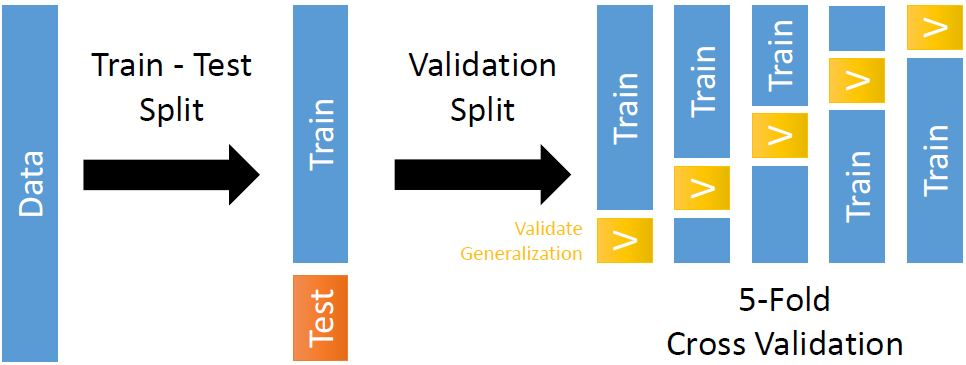
\includegraphics[scale=0.5]{Cattura.JPG}
\end{figure}
Figure 1 from [5] gives a visual representation of the k-fold cross-validation method.

\subsection{Bias-Variance trade-off}
The bias is an important quantity to study since it measures the inability for a machine learning method to capture the true relationship. To calculate it, we measure the distances from the fit lines to the data, square them and add them up.
The variance, on the other hand, measures the difference in fits between data sets. 
In linear regression we normally have a high bias but a low variance, that means that we have predictions that are not great, but consistent.
As the order of the polynomial increases, the bias shrinks and the variance increases which can lead to over fitting.
\\
\\In Machine Learning one of the most difficult but essential topics is the relation between the two quantities mentioned above. Here, we try to explain it in the clearest possible way.
\\
\\First, for OLS, the cost function (2) to minimize is equivalent to the MSE (13): so to obtain the parameters $\beta_j$, we have to minimize this quantity. We can rewrite (14) as:
\begin{equation}
\begin{split}
\mathbb{E}[(Y_{i} - \hat{Y}_i)^2] &= \mathbb{E}[(f(x_i) + \epsilon_i -  \hat{f}(x_i))^2] =\\&=\underbrace{\mathbb{E}[(f(x_i)  -  \hat{f}(x_i))^2]}_{\mathrm{Reducible}} + \underbrace{\mathbb{V}\mathrm{ar}(\epsilon_i)}_{\mathrm{Irreducible}}
\end{split}
\end{equation} 
where $\mathbb{V}\mathrm{ar}(\epsilon_i)=\sigma^2$. \\
\\
The reducible error can be decomposed into squared bias and variance of the estimator $\hat{f}(x)$, respectively:
\begin{equation}
\begin{split}
&\mathbb{E}[(f(x_i)  -  \hat{f}(x_i))^2]  = \\&=\mathbb{E}[(f(x_i)  - \mathbb{E}(\hat{f}(x_i)) + \mathbb{E}(\hat{f}(x_i)) - \hat{f}(x_i))^2]=
\\&=\underbrace{ [\mathbb{E}\hat{f}(x_i) - f(x_i) ]^2}_{[\mathrm{Bias}(\hat{f}(x_i))]^2} + \underbrace{\mathbb{V}\mathrm{ar}[\hat{f}(x_i)]}_{\mathrm{Variance}(\hat{f}(x_i))}
\end{split}
\end{equation}
Hence $\mathbb{E}(MSE)$ may be written as:
\begin{equation}
\begin{split}
 &\sigma^2 + \underbrace{\frac{1}{n}\sum_{i=0}^{n-1}(\mathbb{E}\hat{f}(x_i) - f(x_i) )^2}_{\mathrm{Bias}^2} + \underbrace{\frac{1}{n}\sum_{i=0}^{n-1} \mathbb{V}\mathrm{ar}(\hat{f}(x_i))}_{\mathrm{Variance}} =
\\
=&\sigma^2 + [\mathrm{Bias}(\hat{f})]^2+\mathrm{Variance}(\hat{f})
\end{split}
\end{equation}
Variance and bias are opposing entities, and it is not possible to minimize both simultaneously. Thus, we must choose a trade-off between bias and variance.


\section{Implementation and results in the Franke function case}
Before considering real data, it is interesting to consider a merely pedagogical case study: we employ the Franke function. 
It is a specific function which is defined in the following way:
\begin{align}
f(x,y) &= \frac{3}{4}\exp\left\{\frac{-1}{4}\left[\left(9x-2\right)^2 + \left(9y-2\right)^2\right]\right\}\nonumber \\
%%
&+ \frac{3}{4}\exp\left\{\frac{-1}{49}\left(9x+1\right)^2 + \frac{1}{10}\left(9y+1\right)^2\right\}\nonumber \\
%%
&+ \frac{1}{2}\exp\left\{\frac{-1}{4}\left[\left(9x-7\right)^2 + \left(9y-3\right)^2\right]\right\}\nonumber \\
%%
&- \frac{1}{5}\exp\left\{\frac{-1}{4}\left[\left(9x+4\right)^2 + \left(9y-7\right)^2\right]\right\}.
\end{align}

The function is defined for $x,y$ $\epsilon$ $[0, 1]$.
\\
\\Using this function and randomly chosen $x$ and $y$-values between 0 and 1, we generate a data set of $(x_i,y_i,z_i)$ points with $z_i=f(x_i,y_i)+\epsilon$ where $\epsilon \sim N(0,\sigma^2)$  .\\
Then, the design matrix $\textbf{X}$ is built so that:\\
\begin{equation}
\begin{bmatrix}
x_0^{0}y_0^{0} & x_0^{1}y_0^{0} & x_0^{0}y_0^{1} & ... & x_0^{i}y_0^{j}\\
... & ... & ... & ... & ... \\
x_k^{0}y_k^{0} & x_k^{1}y_k^{0} & x_k^{0}y_k^{1} &  ... & x_k^{i}y_k^{j}\\
... & ... & ... & ... & ... \\
x_{n-1}^{0}y_{n-1}^{0} & x_{n-1}^{1}y_{n-1}^{0} & x_{n-1}^{0}y_{n-1}^{1} &  ... & x_{n-1}^{i}y_{n-1}^{j}\\ 
\end{bmatrix}
\end{equation}
\\with $i+j \leq q$ where $q$ is the degree of the polynomial fit. After that, we create a Python class named \textit{Regression-methods}: given the design matrix \textbf{X}, the $y$-values and a certain value of $\lambda$ ($\lambda=0$ for OLS, otherwise for Ridge regression),
it calculates the $\beta$-coefficients which minimise the associated cost-function and also the confidence interval for them (estimating previously the variance of $\boldsymbol{\hat{\beta}}$).
We then wrote functions to calculate two important error metrics, $MSE$ and $R^2$.
For the Lasso regression, we use the Lasso-method found
in scikit-learn library.
\subsection{OLS}
First we consider the whole data set without resampling. Using the class previously created and fixing $\lambda=0$(OLS) for a polynomial of degree five, we obtain that: 
\begin{center}
\begin{tabular}{ |c|c|c|c| } 
\hline
$MSE$ & $R^2$ \\
\hline
0.00453 & 0.94493 \\ 
\hline
\end{tabular}
\end{center}
$MSE$ is very small and the $R^2$ coefficient of determination is high. Thus the model predicts the true values quite well. Next we calculate the confidence intervals of the $\beta$ coefficients as shown in the table below.

\begin{center}
\begin{tabular}{ |c|c|c|c| } 
\hline
$\beta_j$ & Confidence interval($\alpha=0.1$) \\
\hline
$\beta_0$ & $0.418\pm0.002$\\
$\beta_2$ & $-9.06\pm0.105$\\
... & ...\\
$\beta_{16}$ & $-57.2\pm0.185$\\
$\beta_{18}$ & $-14.6\pm0.234$\\
... & ...\\
\hline
\end{tabular}
\end{center}
The $\beta$-coefficients from OLS do not have a high variance (and consequently small confidence intervals) and do not become unstable since range is small and the noise is not too considerable: thanks to that, small changes in the data do not result in large changes in the model. If the noise was bigger, predictions could be very unstable and one way to mitigate this problem would be to use shrinkage methods such as Ridge regression.
However, we do not want our model to follow the data too closely, losing the global tendency, as this will often result in over-fitting.  
\\
\\
To bypass this, we also study the variance and bias.
Before studying these two different measures we shuffle our original data-set and split it in two parts: training and test data. This means that we set aside 20\% of the data to be used to test our model obtained from the training data. On the remaining data we used the K-fold validation algorithm with $k=5$.
Here, it is interesting to study the relationship between training vs. test error and model complexity (polynomial degree) vs. error metrics such as $MSE$.
\\

\begin{figure}[H]
\caption{Plot representing test and training errors as a function of model complexity for OLS regression}
\centering
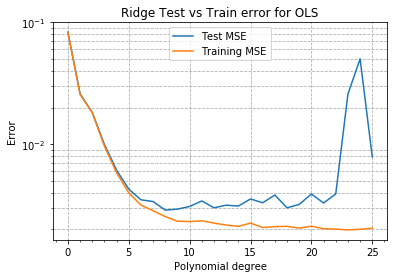
\includegraphics[scale=0.5]{traintest.png}
\label{test_training_OLS}
\end{figure}
\\

The orange curves are test and the blue are training errors for OLS regression.
Figure~\ref{test_training_OLS}  shows the ordinary behaviour of the two errors as model complexity is varied. Increasing the model complexity, the training error tends to drop off.
However, we have to avoid this situation since the model fits itself too strictly to the training data, resulting in a non general solution.
On the other hand, if the model is not complex enough, it under fits since it has a large bias.
\\
\begin{figure}[H]
\caption{The MSE of the model, decomposed
into bias and variance, as a function of polynomial degree }
\centering
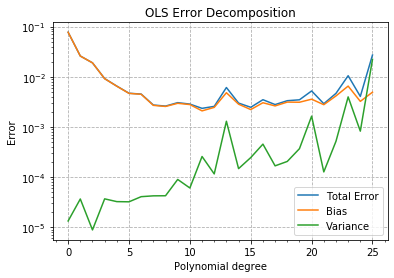
\includegraphics[scale=0.5]{OLS_error_decomposition.png}
\label{bias_variance_OLS_true}
\end{figure}
In Figure ~\ref{bias_variance_OLS_true} we can see the decomposition of the reducible error in bias and variance. As expected, for lower polynomial degrees the bias is high and the variance is not remarkable. For higher degrees the bias is minor (and stable) but the variance starts to reach higher values.

\subsection{Ridge regression}
In order to determine an optimal $\lambda$ for a specific degree Ridge regression model, we compared the MSE of different degree Ridge regression models with varying shrinkage hyperparameters.
\begin{figure}[H]
\caption{The MSE of the model for different polynomial degrees as a function of $\lambda$ }
\centering
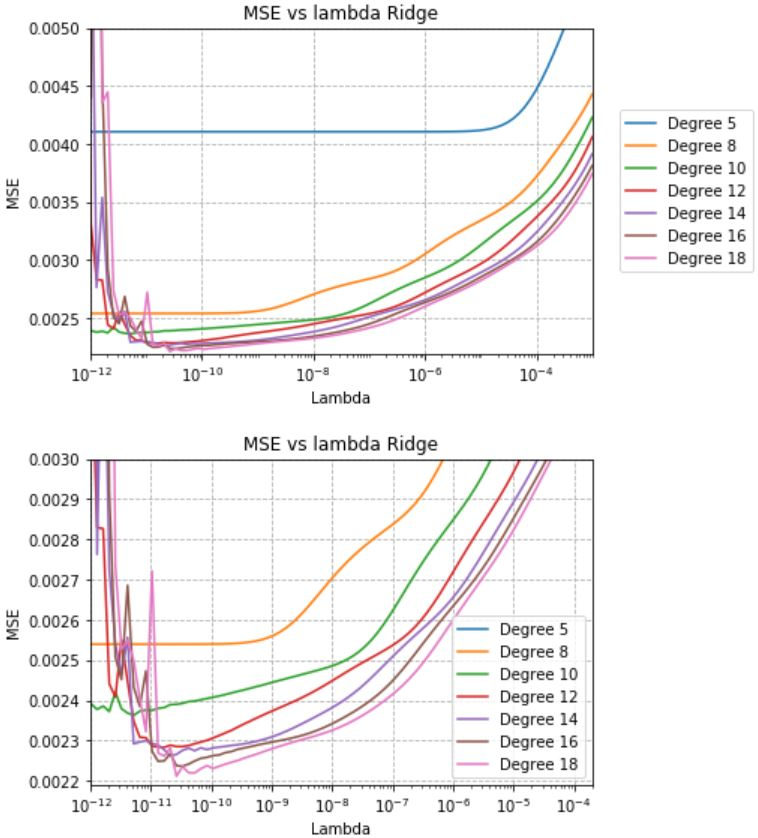
\includegraphics[scale=0.7]{oka.JPG}
\label{MSE_PD_LAM_RID}
\end{figure}
As shown in the first plot in Figure~\ref{MSE_PD_LAM_RID}, the $MSE$ calculated with degree=5 for $\lambda>10^{-11}$ is always bigger than the ones obtained with higher degrees. 
We consider now three different $\lambda$s with degree fixed to five: $10^{-4}$, $10^{-7}$, $10^{-10}$. Here are the results:
\begin{center}
\begin{tabular}{ |c|c|c|c| } 
\hline
$\lambda$ & $MSE$ & $R^2$ \\
\hline
$10^{-4}$ & 0.00562 & 0.93133 \\
$10^{-7}$ & 0.00411 & 0.949863\\ 
$10^{-10}$ & 0.00410 & 0.949865\\
\hline
\end{tabular}
\end{center}
Since $\lambda=10^{-10}$ seems to be the hyperparameter that gives the best MSE, we first calculate the related $\beta$-coefficients (with their relative confidence intervals) and then study the relationship between MSE and polynomial degree.
\begin{center}
\begin{tabular}{ |c|c|c|c| } 
\hline
$\beta_j$ & Confidence interval($\alpha=0.1$) \\
\hline
$\beta_0$ & $0.281\pm0.002$\\
$\beta_2$ & $-9.87\pm0.118$\\
... & ...\\
$\beta_{16}$ & $-58.1\pm0.188$\\
$\beta_{18}$ & $-28.5\pm0.234$\\
... & ...\\
\hline
\end{tabular}
\end{center}
\begin{figure}[H]
\centering
\caption{The MSE decomposition for $\lambda=10^{-10}$ as a function of polynomial degree in Ridge regression}
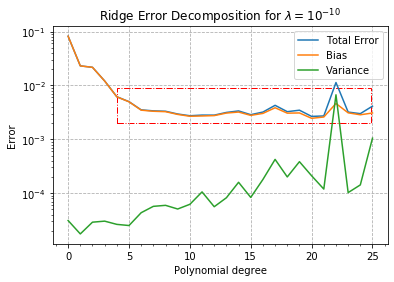
\includegraphics[scale=0.50]{q.png}
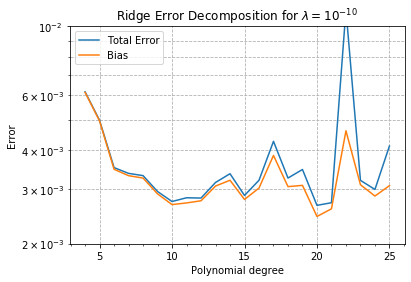
\includegraphics[scale=0.50]{qq.png}
\label{decom_rid}
\end{figure}
We notice in Figure~\ref{decom_rid} that the variance with $\lambda=10^{-10}$ assumes insignificant values meaning that nearly the entirety of the $MSE$ is because of bias. It is also interesting to study the comparison of the $MSE$ values from $OLS$ and ridge.
\begin{figure}[H]
\centering
\caption{$MSE$ for OLS and Ridge with $\lambda=10^{-10}$ as a function of polynomial degree}
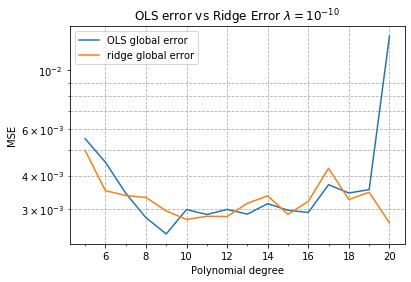
\includegraphics[scale=0.59]{qqqq.png}
\label{OLS_ridge}
\end{figure}
As shown in Figure~\ref{OLS_ridge}, the error obtained by Ridge regression is not so different from the error obtained by $OLS$. We can see that the $MSE$ reaches its minimum with the 9-th degree polynomial for $OLS$. While Ridge regression seems more stable than $OLS$ for higher polynomial degrees. For this particular case, using one over another does not create a significant difference until we fit with polynomials of degree 18 or higher.


\subsection{Lasso regression}
Again the $MSE$ is examined and plotted as a function of the shrinkage factor $\lambda$ (Figure~\ref{mse_lasso}). As in the case with Ridge, the error decreases when the complexity is higher and low values of $\lambda$ seem to give the best $MSE$.
\begin{figure}[h]
    \centering
    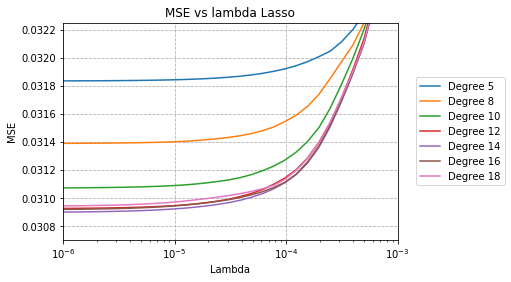
\includegraphics[scale=0.5]{w.png}
    \caption{$MSE$ of the model obtained by Lasso regression for different polynomial degrees as a function of $\lambda$}
    \label{mse_lasso}
\end{figure}
\\Similar to Ridge regression, from Figure~\ref{deco_lasso}  we note that the bias is heavily preponderant in the composition of $MSE$ and the variance increases with the polynomial degree. $\lambda = 5x10^{-6}$ is shown to minimize the error for all plotted degrees.
\begin{figure}[H]
    \centering
    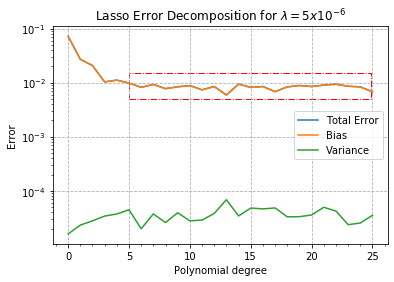
\includegraphics[scale=0.6]{www.png}
    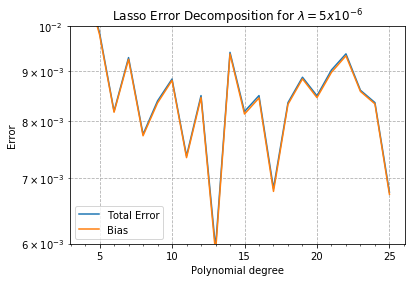
\includegraphics[scale=0.6]{wwww.png}
    \caption{$MSE$ decomposition for $\lambda=5\times10^{-6}$ as a function of polynomial degree in Lasso Regression}
    \label{deco_lasso}
\end{figure}
As shown in Figure~\ref{ols_lasso}, $OLS$ is better than Lasso since $MSE$ is smaller but we can notice that for higher polynomial degrees Lasso is more stable than $OLS$.
\begin{figure}[H]
    \centering
    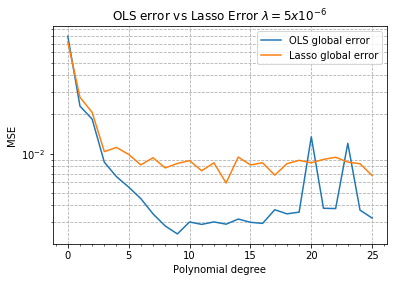
\includegraphics[scale=0.6]{wwwww.png}
    \caption{Comparing MSE for $OLS$ and Lasso with $\lambda=5\times10^{-6}$ as a function of plynomial degree}
    \label{ols_lasso}
\end{figure}
\section{Implementation and results in real terrain data}
In this section we analyse the terrain over Cooke City, Montana.
The terrain is shown in Figure~\ref{maps}.
\begin{figure}[H]
    \centering
    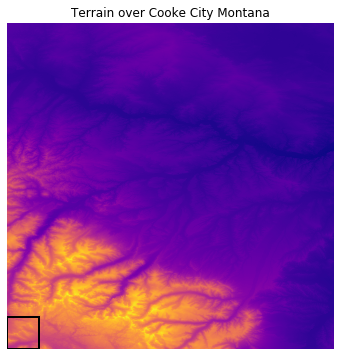
\includegraphics[scale=0.55]{map.png}
    \caption{Picture of terrain with area of interest enclosed in the black box}
    \label{maps}
\end{figure}
From the original data set, we select a patch of dimensions $350\times350$. We then condense this data by selecting every tenth pixel in the $x$ and $y$ directions. Next we make a mesh grid of the $x$ and $y$ points to go with the corresponding z values.

\begin{figure}[H]
\centering
\caption{Plot of terrain data set with $z$ direction measured in meters above sealevel}
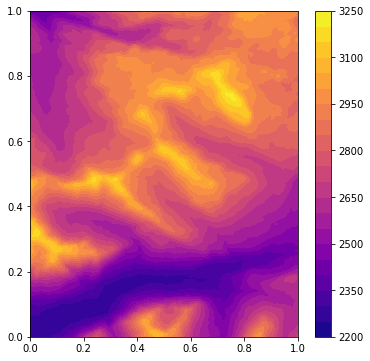
\includegraphics[scale=0.55]{mapgrad.png}
\label{maps1}
\end{figure}
The resulting data set is shown in Figure 11. We will implement all previously discussed methods on this set.
\subsection{OLS}
Here, we apply the same error analysis to the terrain data as was applied to the Franke function.\\
\\
Considering a function of degree five without splitting the data set we obtain: 

\begin{center}
\begin{tabular}{ |c|c|c|c| } 
\hline
$MSE$ & $R^2$ \\
\hline
10461.4986 & 0.7651 \\ 
\hline
\end{tabular}
\end{center}
$MSE$ would seem unreasonably large but it is not since it is a squared quantity that depends directly on the terrain data which is of magnitude $~10^{3}$. 
$R^2$ coefficient of determination is yet another confirmation of a well fitting model, as was shown with the Franke function. 
\begin{center}
\begin{tabular}{ |c|c|c|c| } 
\hline
$\beta_j$ & Confidence interval($\alpha=0.1$) \\
\hline
$\beta_0$ & $2.15\times10^3\pm2.43$\\
$\beta_2$ & $1.23\times10^4\pm1.37\times10^2$\\
... & ...\\
$\beta_{16}$ & $5.74\times10^4\pm2.22\times10^2$\\
... & ...\\
\hline
\end{tabular}
\end{center}
Again, we see that the variance in $\beta$ is small, resulting in narrow confidence intervals.
\begin{figure}[H]
    \centering
    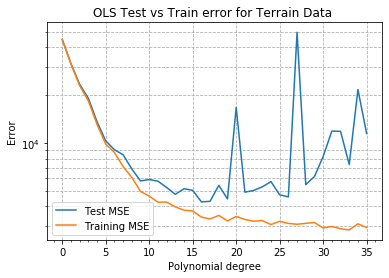
\includegraphics[scale=0.5]{terr1.png}
    \caption{Test and Train error for Terrain Data($OLS$)}
    \label{ma}
\end{figure}
From Figure~\ref{ma} we can see the expected behaviour of test and training $MSE$ as polynomial degree increases.
\begin{figure}[H]
    \centering
    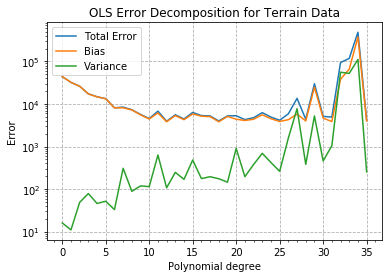
\includegraphics[scale=0.6]{terr2.png}
    \caption{$MSE$ decomposition for Terrain Data using $OLS$}
    \label{OLS_1}
\end{figure}

 In Figure~\ref{OLS_1}, we see that for polynomial degree bigger than 26 the variance plays a more significant role and  the fit becomes unstable. With more polynomial degrees, the model fits to the noise of the training data, resulting in poor results when making predictions with the test data. Our results are consistent with those seen form the Franke function. From Figure~\ref{OLS_1} we see that the $MSE$ is optimized for degree 18.
 
\begin{figure}[H]
    \centering
    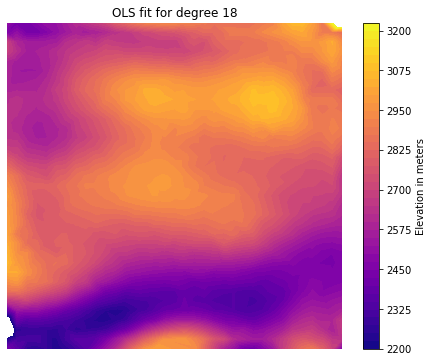
\includegraphics[scale=0.55]{terr3.png}
    \caption{Our terrain data predicted by $OLS$ for degree 18}
    \label{plot_OLS}
\end{figure}
\\
\\Comparing Figure~\ref{maps1} to the image obtained by $OLS$ with a polynomial degree of 18 (Figure~\ref{plot_OLS}) and also analyzing Figure~\ref{error}, we notice that the error between the regression predictions and the true terrain data values are not large. As expected, the errors are more prevalent in the areas where the elevation becomes much higher and much lower with respect the to the average, respectively underestimating and overestimating.
\begin{figure}[H]
    \centering
    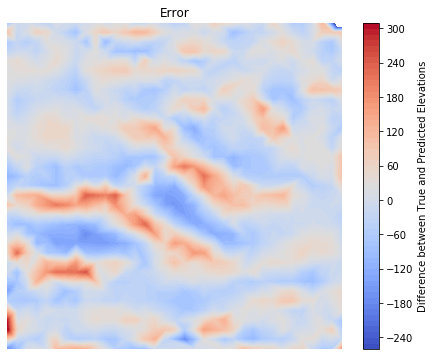
\includegraphics[scale=0.55]{terr4.png}
    \caption{Picture representing the difference between true and predicted elevations}
    \label{error}
\end{figure}

\subsection{Ridge regression}
As observed with the Franke function, the $MSE$ tends to get higher when the $\lambda$ increases and the polynomial degree is low. For the higher degrees, we notice that $MSE$ reaches a minimum around $\lambda=2\times10^{-9}$.
\begin{figure}[H]
    \centering
    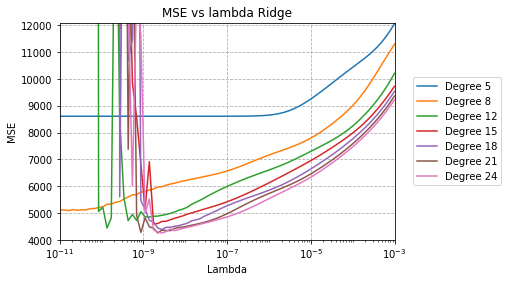
\includegraphics[scale=0.5]{terr5.png}
    \caption{$MSE$ for different polynomial degrees as a function of $\lambda$}
    \label{ridge_terr_1}
\end{figure}
Considering $\lambda=2\times10^{-9}$ and performing the same analysis as previously done, we obtain the results summarised by the two plots in Figure~\ref{ridge_terr_2}. The variance is small and almost the totality of the $MSE$ is due to the bias. From the plots we see that the error is optimized when a polynomial of degree 23 is considered.
\begin{figure}[H]
    \centering
    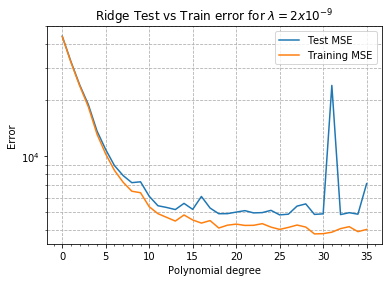
\includegraphics[scale=0.55]{terr6.png}
    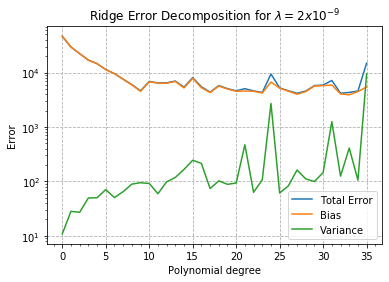
\includegraphics[scale=0.55]{terr7.png}
    \caption{$MSE$ decomposition for Ridge with $\lambda=2\times10^{-9}$}
    \label{ridge_terr_2}
\end{figure}
Comparing the $OLS$ results in Figures~\ref{plot_OLS},~\ref{error} and the Ridge results in Figures~\ref{ridge_terr_3} and~\ref{ridge_terr_34}, it seems that we do not get important differences when using one or the other.
\begin{figure}[H]
    \centering
    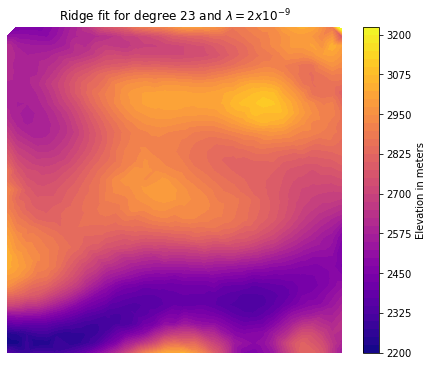
\includegraphics[scale=0.55]{terr9.png}
    \caption{Our terrain data predicted by Ridge regression for degree 23 with $\lambda=2\times10^{-9}$ }
    \label{ridge_terr_3}
\end{figure}
\begin{figure}[H]
\centering
    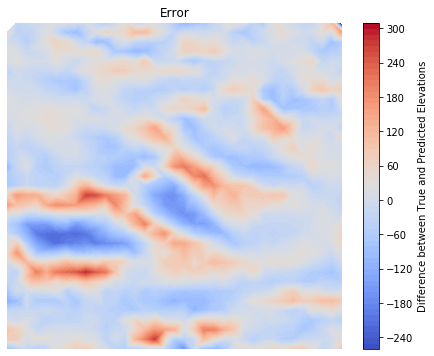
\includegraphics[scale=0.55]{terr10.png}
    \caption{Error plot computed for Ridge regression for degree 23 with $\lambda=2\times10^{-9}$ }
    \label{ridge_terr_34}
\end{figure}
As shown in Figure~\ref{ridge_terr_4}, the error with the Ridge regression appears comparable to the error obtained by $OLS$ when considering polynomial degrees less than 25. We can assert that the MSE reaches its minimum values when $OLS$ is considered; however, Ridge regression is more stable than $OLS$ with higher model complexity.

\begin{figure}[H]
    \centering
    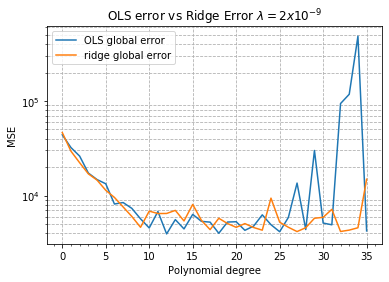
\includegraphics[scale=0.55]{terr8.png}
    \caption{$MSE$ for $OLS$ and Ridge with $\lambda=2\times10^{-9}$ }
    \label{ridge_terr_4}
\end{figure}
\subsection{Lasso regression}
As shown in Figure~\ref{lassoterr1}, we observe a similar tend as was seen when considering Ridge regression. The error decreases when the complexity is higher and $\lambda$ is small. When comparing Figure 20 to Figure 16, we can see that the error for Lasso is a factor of $10^{2}$ higher than for Ridge.  
\begin{figure}[H]
    \centering
    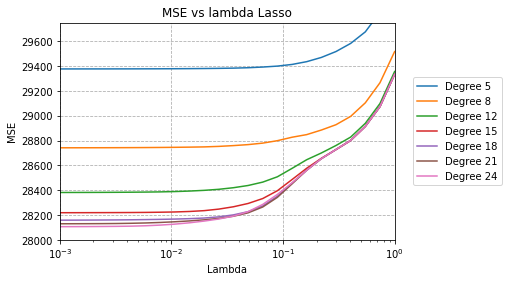
\includegraphics[scale=0.55]{terr11.png}
    \caption{$MSE$ for different polynomial degrees as a function of $\lambda$ using Lasso}
    \label{lassoterr1}
\end{figure}
$\lambda = 6\times10^{-3}$ appears to be a good choice for the polynomial degrees plotted as the MSE has is minimized for this value.
\begin{figure}[H]
    \centering
    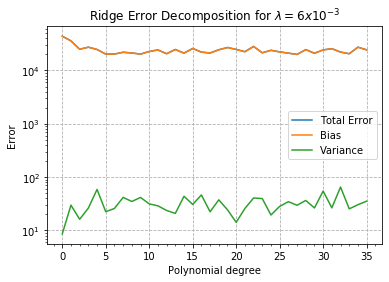
\includegraphics[scale=0.55]{terr14.png}
    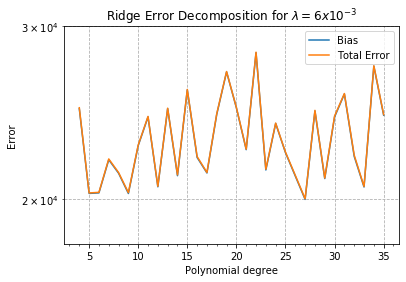
\includegraphics[scale=0.55]{terr15.png}
    \caption{$MSE$ decomposition for Lasso with $\lambda=6\times10   ^{-3}$}
    \label{lassoterr2}
\end{figure}
In Figure~\ref{lassoterr2} we see that the variance does not grow significantly and so the total error almost entirely due to the bias of the model.
\begin{figure}[H]
    \centering
    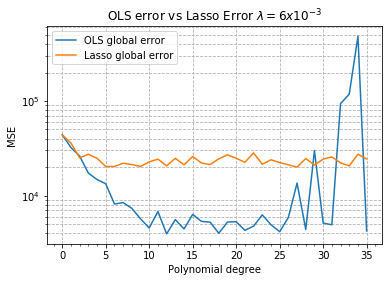
\includegraphics[scale=0.55]{terr16.png}
    \caption{$MSE$ for $OLS$ and Lasso with $\lambda=6\times10   ^{-3}$}
    \label{lassoterr3}
\end{figure}
As expected, the $MSE$ due to Lasso regression is higher than the $MSE$ calculated with $OLS$ but we notice that Lasso begins to perform better than $OLS$ when considering higher order polynomials.
From Figure 22, $MSE$ for Lasso is optimized for degree 27. From the following plots, we notice that this model obtained by Lasso regression is far worse than the other models computed by $OLS$ and Ridge.
\begin{figure}[H]
    \centering
    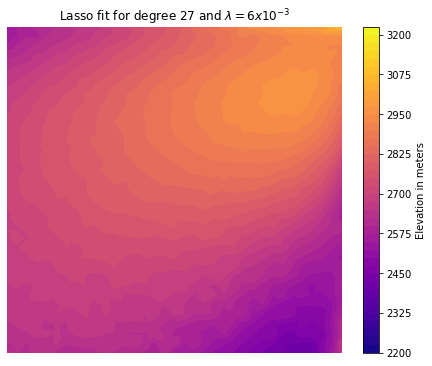
\includegraphics[scale=0.5]{terr17.png}
    \caption{Our terrain data predicted by Lasso regression }
    \label{lassoterr4}
\end{figure}
\begin{figure}[H]
    \centering
    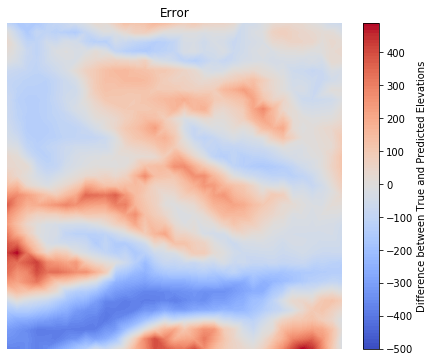
\includegraphics[scale=0.5]{terr18.png}
    \caption{Error plot for Lasso predictions}
    \label{lassoterrex}
\end{figure}
\section{Conclusions}
The results in this project show that for both the Franke function and the studied terrain data, the $OLS$ fits are superior to the regularized Ridge and Lasso fits. We can justify this in both of the cases we studied because bias always prevailed in the decomposition of the MSE, so the variance barely effected the total error. 
This suggests that Ridge Lasso methods, which are variance-reducing regularization regression methods, may not be as effective.
With the data set built with the Franke function, all three methods provided satisfying predictions. With terrain data, $OLS$ and Ridge regression provided much better results than Lasso regression.
One reason could be that Lasso fit forced too many  of the $\beta$-coefficients to zero, thus resulting in a model that misses important information when making predictions. However, we can not ignore that Ridge regression provided good results. This could imply that some of the parameters are more important than others for the construction of the model. 
\subsection{Further research}
In this letter we have focused on three different regression models, often with specific polynomial degrees and $\lambda$. However, similar analysis can be done for several other polynomial degrees, or different regression methods. Perhaps the best path forward would be to also consider logistic regression and compare it to the methods we studied in this letter. 
\pagebreak

\begin{thebibliography}{}
\bibitem{} Hjorth-Jensen, Morten \,Lectures notes in FYS-STK4155.Data analysis and
machine learning: Linear regression and more advanced regression analysis,
Sep 13 2019, https://github.com/CompPhysics/MachineLearning

\bibitem {}Pankaj Mehta, A high-bias, low-variance introduction to Machine Learning for physicists, May 29, 2019
\bibitem {}Trevor Hastie, Robert Tibshirani, and JH Friedman. The elements of statistical learning: data
mining, inference, and prediction. 2009.
\bibitem{} Piccolo Domenico, Statistica, 21 Oct 2010.
\bibitem{}Würsch Christoph, Machine Learning:
\\Bias-Variance-Tradeoff(pptx presentation)
\end{thebibliography}

\section{Appendix}
All source code, data and figures can be found at the github repository: https://github.com/bruce-chappell/FYS4155/tree/master/project1
\end{document}